%%%%%%%%%%%%%%%%%%%%%%%%%%%%%%%%%%%%%%%%%%%%%%%%%%%%
\documentclass[fleqn,10pt,twocolumn]{AROB}

\usepackage[utf8]{inputenc}
\usepackage{amsmath}
\usepackage{xeCJK}
\usepackage{svg}
\setCJKmainfont{Hiragino Mincho ProN}

\title{Blood Pressure Estimation Based on Asymmetric Sine Wave Model Residuals Optimized for PPG in 30fps Visible Camera Environment}

\author{Yusuke Nakazawa${}^{1\dagger}$, Kento Nagumo${}^{1}$, Akio Nozawa${}^{1}$}
% The dagger symbol indicates the presenter.
\speaker{Yusuke Nakazawa}

\affils{${}^{1}$Department of Electrical and Electronic Engineering, Graduate School of Science and Engineering, Aoyama Gakuin University\\
(Tel: 080-5326-3916; E-mail: nynynakazawa@gmail.com)\\
}

\abstract{%
We propose a novel blood pressure estimation method that does not depend on frequency decomposition for pseudo-PPG derived from smartphone visible cameras. In a low sampling rate environment of 30fps, conventional frequency analysis approaches struggle to accurately extract high-order harmonics. In this study, we adopt an existing morphological feature approach (RTBP: RealTimeBloodPressure) as a baseline and implement and compare two newly proposed methods. First is a linear regression model (sinBP(M): sinBP(Model)) that directly uses sine wave fit parameters (amplitude, phase, mean) as features. Second is a three-stage estimation model (sinBP(D): sinBP(Distortion)) that uses the residual (distortion index E) from a physiologically plausible asymmetric sine wave model as a feature. sinBP(M) and sinBP(D) extract essential characteristics of the PPG waveform and realize stable blood pressure estimation that is less susceptible to noise. The evaluation of this study compares three different blood pressure estimation methods (RTBP, sinBP(M), sinBP(D)) using an rPPG environment with a 30fps visible camera, with a continuous blood pressure monitor as a reference, to verify the superiority of the novel methods.
}

\keywords{%
Blood pressure estimation, Photoplethysmography, Smartphone, Asymmetric sine wave model, Distortion index
}

\begin{document}

\maketitle

%-----------------------------------------------------------------------

\section{Introduction}

Continuous non-invasive blood pressure monitoring is essential for the early detection and management of cardiovascular diseases \cite{ref1,ref2}. In recent years, blood pressure estimation using photoplethysmography (PPG) from smartphone visible cameras has attracted attention \cite{ref3}. However, smartphone cameras have a low frame rate of 30fps and are susceptible to illumination fluctuations and noise specific to visible light. Due to these constraints, morphological analysis relying on minute feature points (peaks and TTP) and frequency analysis requiring high-order harmonics are vulnerable to phase fluctuations and the like \cite{ref4,ref5}.

Conventional PPG blood pressure estimation is mainly classified into (1) morphological features (peaks, TTP, etc.) \cite{ref6}, (2) frequency analysis (FFT, etc.) \cite{ref7}, and (3) machine learning (deep learning, etc.) \cite{ref8}. However, in a 30fps environment, sampling points are coarse and cannot capture minute shape changes, making point-dependent morphological features unstable. Also, the Nyquist frequency is low (15Hz), making frequency analysis difficult.

Therefore, in this study, we focus on the "Shape of the entire waveform" rather than individual points or frequency components. We hypothesized that by fitting a model function using all data points for one beat, even in a low FPS and high noise environment of 30fps, local noise and sampling deviations can be smoothed out, enabling robust feature extraction.

Specifically, we propose an asymmetric sine wave model that considers the asymmetry of the systolic and diastolic phases. The steep rise and gradual decay specific to PPG \cite{ref11}, which cannot be represented by a simple sine wave, are approximated by a model with different time scales for the systolic and diastolic phases. The parameters obtained by fitting to this model reflect physiological characteristics as follows.

First, Amplitude ($A$) reflects the flexibility (distensibility) of blood vessels and the stroke volume of blood \cite{ref3,ref11}.
Second, Relative TTP, which indicates the sharpness of the waveform, captures the phenomenon where the reflected wave returns earlier as blood vessels become stiffer (increase in pulse wave velocity) and serves as an indicator of arteriosclerosis \cite{ref6,ref14}.
Third is the "Deviation (Residual $E$)" from the smooth model waveform. This quantifies minute distortion components (such as dicrotic notches) that cannot be represented by the model and is considered to reflect characteristics of vascular aging known in acceleration plethysmogram (APG) analysis \cite{ref13}.
Finally, the interaction term ($E\sqrt{A}$) considering the nonlinearity of the pressure-volume relationship of blood vessels \cite{ref15}. Since blood vessels have the characteristic of becoming stiffer as blood pressure increases (amplitude increases), weighting the distortion $E$ with the amplitude $A$ captures this nonlinear stiffening characteristic.

The purpose of this study is to verify the effectiveness of the novel method using the asymmetric sine wave model. Specifically, we implement and compare the following three methods. Note that since it has been shown that a linear relationship exists between PPG features and blood pressure \cite{ref6,ref9,ref10}, we adopt Ridge regression with a regularization term considering multicollinearity in all methods \cite{ref12}.

\noindent
(1) RTBP: A method using existing morphological features (amplitude, heart rate, relative TTP) \cite{ref6}. This is compared as a baseline.\\[0.5em]
(2) sinBP(M): A method using parameters of the proposed model (asymmetric sine wave model) (amplitude, phase, mean) as features.\\[0.5em]
(3) sinBP(D): A method based on RTBP that uses the residual (distortion) from the proposed model and the vascular stiffness index ($E\sqrt{A}$) as features.

The main contributions of this study are as follows.
First, we proposed a novel approach sinBP(M/D) of "asymmetric sine wave model fitting method" that enables stable feature extraction even in a low-quality video environment of 30fps. Unlike the conventional method (RTBP) that relies on point measurement, this approach enhances robustness to noise by utilizing the entire waveform shape.
Second, we presented a novel approach sinBP(D) that utilizes "deviation (residual)" from a physiological model as an indicator of vascular stiffening. We constructed a framework to model the residual, which is often treated as mere error, as important physiological information (distortion) in blood pressure estimation.
Third, we verified the effectiveness of each method through rigorous comparative experiments using clinical-grade measurement instruments. We quantitatively evaluate how model parameters capturing the basic structure and residuals capturing minute changes contribute to blood pressure estimation, respectively.

%-----------------------------------------------------------------------

\section{Methods}

\subsection{Asymmetric Sine Wave Model}
The PPG waveform has an asymmetry with a short systolic phase and a long diastolic phase \cite{ref15}. In this study, we define an asymmetric sine wave model (Equation \ref{eq:asymmetric_model}) reflecting this characteristic.
\begin{equation}
s(t) = \text{mean} + A \cdot s_{\text{norm}}(t)
\label{eq:asymmetric_model}
\end{equation}

\begin{equation}
s_{\text{norm}}(t) = \frac{1 + \cos(\theta(t) + \phi_0)}{2}
\label{eq:asymmetric_norm}
\end{equation}

\begin{equation}
\theta(t) = \begin{cases}
\frac{3\pi}{2} \cdot \frac{t'}{T} & (0 \leq t' \leq \alpha T) \\
\pi + 3\pi \cdot \frac{t' - \alpha T}{T} & 
(\alpha T < t' \leq T)
\end{cases}
\label{eq:asymmetric_theta}
\end{equation}

Here, $A$ is amplitude, mean is the average value, and $T$ is the period (IBI). $t' = (t - \tau^*) \bmod T$ is the phase time within one beat, $\phi_0$ is a small phase shift, and $\tau^*$ is a parameter for aligning peak positions for each beat. Also, $\alpha$ is a parameter representing the ratio of the systolic phase, and we assume $\alpha \approx 1/3$ (diastolic phase is $1-\alpha \approx 2/3$) as an initial value.

In implementation, the systolic/diastolic ratio is automatically calculated from the measured data of the previous beat by 1-beat delay processing, and the model parameter $\alpha$ is dynamically determined based on that ratio. As a default value, a ratio where peak $\to$ valley is about 2/3 of the period and valley $\to$ next peak is about 1/3 is used, but a dynamic ratio calculated from measured data is used for each beat.

\subsection{Blood Pressure Estimation Methods}
In this study, we compare the following three methods. Ridge regression is used in all methods.

\subsubsection{RTBP (Baseline)}
This is a method using only existing morphological features \cite{ref6}. Amplitude $A$, heart rate HR, and relative TTP (V2P, P2V) are used as features.
\begin{equation}
\begin{split}
\text{SBP}_{\text{RTBP}}&= C_0 + C_1 \cdot A + C_2 \cdot \text{HR} \\
&\quad + C_3 \cdot \text{V2P\_relTTP} + C_4 \cdot \text{P2V\_relTTP}
\end{split}
\label{eq:rtbp_sbp}
\end{equation}

\begin{equation}
\begin{split}
\text{SBP}_{\text{RTBP}}&= D_0 + D_1 \cdot A + D_2 \cdot \text{HR} \\
&\quad + D_3 \cdot \text{V2P\_relTTP} + D_4 \cdot \text{P2V\_relTTP}
\end{split}
\label{eq:rtbp_dbp}
\end{equation}

\subsubsection{sinBP(M) (Proposed Method 1)}
This is a method using model parameters directly as features. Amplitude $A$, heart rate HR, mean value Mean, and phase $\Phi$ are used as features.
\begin{equation}
\begin{split}
\text{SBP}_{\text{Model}}&= \alpha_0 + \alpha_1 \cdot A + \alpha_2 \cdot \text{HR} \\
&\quad + \alpha_3 \cdot \text{Mean} + \alpha_4 \cdot \Phi
\end{split}
\label{eq:sinbp_m_sbp}
\end{equation}

\begin{equation}
\begin{split}
\text{DBP}_{\text{Model}} &= \beta_0 + \beta_1 \cdot A + \beta_2 \cdot \text{HR} \\
&\quad + \beta_3 \cdot \text{Mean} + \beta_4 \cdot \Phi
\end{split}
\label{eq:sinbp_m_dbp}
\end{equation}

\subsubsection{sinBP(D) (Proposed Method 2)}
This is a method using model residual (distortion) as a feature. In addition to $A$, HR, and relative TTP, Stiffness\_sin ($E\sqrt{A}$) and distortion $E$ are used.
Distortion index $E$ is the RMS error between the measured waveform $x[n]$ and the model waveform $s[n]$ (Equation \ref{eq:distortion}).
\begin{equation}
E = \sqrt{\frac{1}{N} \sum_{n=1}^{N} (x[n] - s[n])^2}
\label{eq:distortion}
\end{equation}

Furthermore, the product of the distortion index $E$ and the square root of the amplitude $A$ is defined as the vascular stiffness index Stiffness\_sin:
\begin{equation}
\text{Stiffness}_{\text{sin}} = E \sqrt{A}
\label{eq:stiffness}
\end{equation}

Estimation is performed in two stages: (1) Base BP + Vascular characteristic correction (RTBP + Stiffness), (2) Distortion correction (+$E$).

[Stage 1: Base BP + Vascular characteristic correction]
\begin{equation}
\begin{split}
\text{SBP}_{\text{vascular}} &= \text{SBP}_{\text{RTBP}} \\
&\quad + \text{ALPHA}_5 \cdot \text{Stiffness}_{\text{sin}}
\end{split}
\label{eq:sinbp_d_sbp_model}
\end{equation}

\begin{equation}
\begin{split}
\text{DBP}_{\text{vascular}} &= \text{DBP}_{\text{RTBP}} \\
&\quad + \text{BETA}_5 \cdot \text{Stiffness}_{\text{sin}}
\end{split}
\label{eq:sinbp_d_dbp_model}
\end{equation}

[Stage 2: Distortion correction]
\begin{equation}
\text{SBP}_{\text{Distortion}} = \text{SBP}_{\text{vascular}} + \text{ALPHA}_6 \cdot E
\label{eq:sinbp_d_sbp_final}
\end{equation}

\begin{equation}
\text{DBP}_{\text{Distortion}} = \text{DBP}_{\text{vascular}} + \text{BETA}_6 \cdot E
\label{eq:sinbp_d_dbp_final}
\end{equation}

\subsection{Preprocessing}
Peak detection, beat segmentation, time normalization ($N=64$), peak alignment (phase search), and outlier removal (IBI, amplitude fluctuation) are performed.

%-----------------------------------------------------------------------

\section{Experiment Plan}
\subsection{Protocol}
\subsubsection{Environment Settings}
A Google Pixel 8 front visible camera (30fps) was used as the device, and measurement was performed using the finger pad contact method (index finger). Lighting conditions were set to 400 lux indoors.

\subsubsection{Reference Values}
As a reference device, real-time PPG was simultaneously measured at the fingertip cuff (middle finger) with an optical pulse oximeter (IWS920-DEV, resolution 409.6Hz). Also, real-time blood pressure was simultaneously measured at the fingertip cuff (middle finger/ring finger) with a continuous blood pressure monitor (CNAP-Monitor, resolution 1000Hz, clinical grade). As measurement conditions, measurement interval, body position, and rest time were unified.

\subsubsection{Subjects}
The subjects were 5 healthy adult males aged 20-23, with exclusion criteria such as severe arrhythmia. Measurement was performed 3 times for each subject.

\subsubsection{Ethics}
Informed consent, anonymization, and encrypted storage are implemented.

\subsection{Evaluation Metrics}
In this study, evaluation is performed using the following metrics. First, as waveform evaluation, the reference waveform and smartphone waveform (Green/sinWave) are time-synchronized and evaluated by MAPE, MAE, and correlation coefficient. Next, regarding blood pressure estimation accuracy, 5-fold time series cross-validation is used to compare and verify the three methods using MAE, RMSE, and MAPE. At that time, AAMI criteria ($|\text{MD}|\leq 5, \text{SD}\leq 8$) are also referred to. Furthermore, as an ablation study, the contribution of each feature is evaluated by coefficient analysis.

\section{Results}
\subsection{Waveform Evaluation}
Table \ref{tab:waveform_eval} shows the waveform evaluation results. sinWave improved by about 11.5 points in MAPE compared to Green, and the correlation coefficient also improved. This indicates that model approximation functioned as noise removal.

\begin{table}[h]
\caption{Waveform evaluation results (Average of all sessions)}
\label{tab:waveform_eval}
\centering
\small
\begin{tabular}{lccccc}
\hline
Channel & MAPE [\%] & MAE & RMSE & Bias & Corr \\
\hline
sinWave & 18.22 & 1.82 & 2.24 & -0.66 & 0.19 \\
Green & 29.71 & 2.97 & 3.64 & +0.42 & 0.07 \\
\hline
\end{tabular}
\end{table}

\subsection{Blood Pressure Estimation Accuracy}
Tables \ref{tab:sbp_acc} and \ref{tab:dbp_acc} show the estimation accuracy. The proposed method sinBP(D) achieved the minimum MAE/RMSE for both SBP/DBP. In particular, the improvement in RMSE is remarkable, indicating that large errors can be suppressed.

\begin{table}[h]
\caption{SBP estimation accuracy}
\label{tab:sbp_acc}
\centering
\small
\begin{tabular}{lccc}
\hline
Method & MAPE [\%] & MAE [mmHg] & RMSE [mmHg] \\
\hline
sinBP(D) & 16.44 & 18.98 & 24.17 \\
sinBP(M) & 16.92 & 19.47 & 24.70 \\
RTBP & 17.82 & 20.66 & 28.02 \\
\hline
\end{tabular}
\end{table}

\begin{table}[h]
\caption{DBP estimation accuracy}
\label{tab:dbp_acc}
\centering
\small
\begin{tabular}{lccc}
\hline
Method & MAPE [\%] & MAE [mmHg] & RMSE [mmHg] \\
\hline
sinBP(D) & 21.72 & 14.84 & 19.31 \\
sinBP(M) & 22.30 & 15.20 & 19.73 \\
RTBP & 23.14 & 16.11 & 22.43 \\
\hline
\end{tabular}
\end{table}

\begin{figure*}[t]
\centering
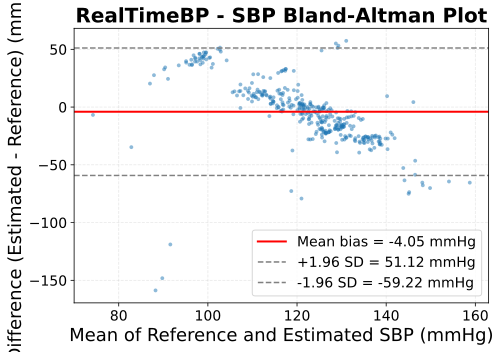
\includegraphics[width=0.32\textwidth]{figures/RealTimeBP_SBP_bland_altman.png}
\hfill
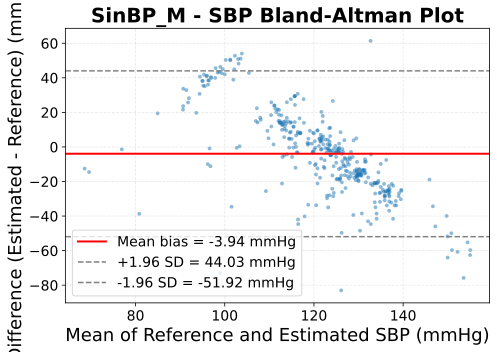
\includegraphics[width=0.32\textwidth]{figures/SinBP_M_SBP_bland_altman.png}
\hfill
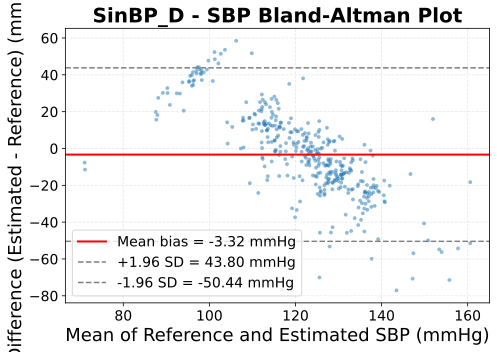
\includegraphics[width=0.32\textwidth]{figures/SinBP_D_SBP_bland_altman.png}
\caption{Bland-Altman plots of SBP. Left: RTBP, Center: sinBP(M), Right: sinBP(D).}
\label{fig:sbp_ba_all}
\end{figure*}

\begin{figure*}[t]
\centering
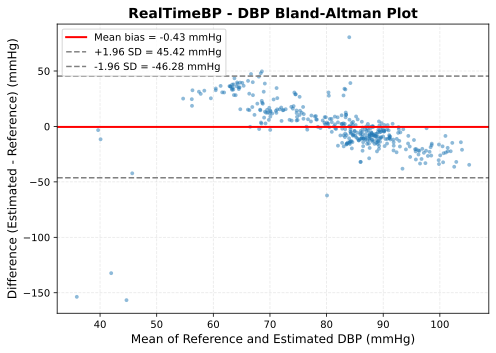
\includegraphics[width=0.32\textwidth]{figures/RealTimeBP_DBP_bland_altman.png}
\hfill
\includegraphics[width=0.32\textwidth]{figures/SinBP_M_DBP_bland_altman.png}
\hfill
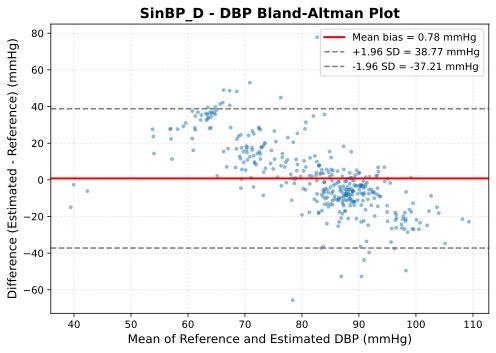
\includegraphics[width=0.32\textwidth]{figures/SinBP_D_DBP_bland_altman.png}
\caption{Bland-Altman plots of DBP. Left: RTBP, Center: sinBP(M), Right: sinBP(D).}
\label{fig:dbp_ba_all}
\end{figure*}

\begin{figure}[t]
\centering
\includegraphics[width=0.49\linewidth]{figures/comparison_SBP_barplot_MAE.png}
\hfill
\includegraphics[width=0.49\linewidth]{figures/comparison_SBP_barplot_RMSE.png}
\\[0.5em]
\includegraphics[width=0.49\linewidth]{figures/comparison_SBP_barplot_MAPE.png}
\caption{Comparison of SBP estimation accuracy across three methods (RTBP, sinBP(M), sinBP(D)). Top left: MAE, Top right: RMSE, Bottom: MAPE.}
\label{fig:sbp_comp}
\end{figure}

\begin{figure}[t]
\centering
\includegraphics[width=0.49\linewidth]{figures/comparison_DBP_barplot_MAE.png}
\hfill
\includegraphics[width=0.49\linewidth]{figures/comparison_DBP_barplot_RMSE.png}
\\[0.5em]
\includegraphics[width=0.49\linewidth]{figures/comparison_DBP_barplot_MAPE.png}
\caption{Comparison of DBP estimation accuracy across three methods (RTBP, sinBP(M), sinBP(D)). Top left: MAE, Top right: RMSE, Bottom: MAPE.}
\label{fig:dbp_comp}
\end{figure}

Contribution of features in sinBP(D):
In sinBP(D), the distortion index E had a large positive coefficient for both SBP and DBP (SBP: +14.88, DBP: +15.20). This indicates that there is a tendency for blood pressure to be higher as the waveform distortion is larger, which is consistent with the physiological finding that arteriosclerosis and increased vascular resistance appear as waveform distortion.
On the other hand, the vascular stiffness index Stiffness\_sin ($E\sqrt{A}$) showed a negative coefficient (SBP: -2.40, DBP: -3.44). This suggests that not only the distortion alone but also the interaction term with amplitude functions as a correction.

Contribution of features in sinBP(M):
In sinBP(M), it was confirmed that the phase Phi has a positive coefficient (SBP: +11.79, DBP: +15.69) and contributes significantly to blood pressure estimation. This supports the fact that pulse wave velocity and the timing (phase) of reflected waves are closely related to blood pressure.

\section{Discussion}

\subsection{Interpretation of Results}

The results of this study strongly support that the approximation approach using the asymmetric sine wave model, which does not depend on frequency analysis, is effective in a low sampling rate environment of 30fps.

First, the fact that the sinWave channel showed higher accuracy (lower MAPE) than the Green channel in waveform evaluation means that the asymmetric sine wave model functioned as a noise removal and waveform shaping filter, extracting the basic components of PPG. Although the raw Green signal is directly affected by illumination fluctuations and body motion noise, it is considered that by performing model approximation, regression to a physiologically plausible "ideal waveform" was performed, and the S/N ratio improved.

Next, the fact that sinBP(D) achieved the highest accuracy in blood pressure estimation indicates that "deviation (residual) from the physiological model" holds important information in blood pressure estimation. It is inferred that by not only parameterizing the waveform (sinBP(M)) but also quantifying the "distortion" that cannot be fully explained by that model and incorporating it as a feature, minute physiological changes such as vascular stiffness and changes in peripheral resistance could be captured.

\subsection{Superiority of Method}

The existing method (RTBP) relied on "point" information such as peaks and valleys of the waveform, so accurate feature extraction was difficult with a coarse time resolution of 30fps (sampling points deviate from peaks, etc.). In contrast, the proposed method (sinBP series) performs least squares fitting using all data points for one beat, so it is robust against sampling timing deviations. This is considered the main factor why sinBP(M) and sinBP(D) outperformed RTBP.

Furthermore, the fact that sinBP(D) outperformed sinBP(M) demonstrates the effectiveness of the "physiological constraint" of the asymmetric sine wave model. It is considered that the correlation with blood pressure increased because the residual (E) of the asymmetric model considering the systolic/diastolic ratio reflects pure "pathological/physiological distortion" better than simple parameter extraction (sinBP(M)).

\subsection{Limitations and Future Prospects}
MAPE is in the 16\% range and has not reached the AAMI criteria. In the future, it is necessary to work on (1) individual difference correction (calibration), (2) model extension (addition of second harmonic), and (3) expansion of the dataset.

\section{Conclusion}
In this study, we proposed a blood pressure estimation method using an asymmetric sine wave model for a 30fps visible camera environment. As a result of the experiment, sinBP(D) using model residuals showed the highest accuracy, and the effectiveness of the distortion index reflecting vascular stiffening was confirmed.

The main contributions of this study are as follows. First, as the utility of sinBP(M), we showed that parameters (amplitude, phase, mean) obtained by fitting to an asymmetric sine wave model function as robust features against noise even in a 30fps environment. Second, as the novelty of sinBP(D), we improved blood pressure estimation accuracy by characterizing "deviation (residual)" from a physiologically plausible model, capturing vascular stiffening and changes in peripheral resistance. In particular, we confirmed that the combination of distortion index $E$ and amplitude $A$ (Stiffness\_sin) is effective. Third, as the feasibility in low FPS environment, we demonstrated that practical blood pressure trend estimation is possible even with a general smartphone camera (30fps) by time-domain modeling that does not depend on frequency decomposition.

This method is expected to contribute to the mHealth field as a simple blood pressure monitoring technology that does not require dedicated devices. In the future, we aim for practical application by proceeding with the introduction of individual difference correction and verification with large-scale datasets.
%%%%%%%%%%%%%%%%% BIBLIOGRAPHY IN THE LaTeX file !!!!! %%%%%%%%%%%%%%%%%%%%%%
\begin{thebibliography}{15}
\bibitem{ref1}
World Health Organization. "Global report on hypertension 2023: the race against a silent killer." Geneva: World Health Organization, 2023.

\bibitem{ref2}
Whelton, Paul K., et al. "2017 ACC/AHA Guideline for the Prevention, Detection, Evaluation, and Management of High Blood Pressure in Adults." \textit{Journal of the American College of Cardiology}, vol. 71, no. 19, 2018, pp. e127-e248.

\bibitem{ref3}
Sun, Yu, and Nitish Thakor. "Photoplethysmography revisited: from contact to noncontact, from point to imaging." \textit{IEEE Transactions on Biomedical Engineering}, vol. 63, no. 3, 2016, pp. 463-477.

\bibitem{ref4}
Verkruysse, Wim, Lars O. Svaasand, and J. Stuart Nelson. "Remote plethysmographic imaging of skin perfusion." \textit{Optics Express}, vol. 16, no. 26, 2008, pp. 21434-21445.

\bibitem{ref5}
McDuff, Daniel, et al. "Improvements in remote cardiopulmonary measurement using a five band camera." \textit{IEEE Transactions on Biomedical Engineering}, vol. 61, no. 10, 2014, pp. 2593-2601.

\bibitem{ref6}
Millasseau, Sandrine C., et al. "Contour analysis of the photoplethysmographic pulse measured at the finger." \textit{Journal of Hypertension}, vol. 24, no. 8, 2006, pp. 1449-1456.

\bibitem{ref7}
Alian, Aymen A., and Kirk H. Shelley. "Photoplethysmography." \textit{Best Practice \& Research Clinical Anaesthesiology}, vol. 28, no. 4, 2014, pp. 395-406.

\bibitem{ref8}
Zhang, Liang, et al. "Developing personalized models of blood pressure estimation from wearable sensors data using minimally-trained domain adversarial neural networks." \textit{Proceedings of Machine Learning Research}, vol. 126, 2020, pp. 97-120.

\bibitem{ref9}
Charlton, Peter H., et al. "Assessing model age from the photoplethysmogram: a systematic review." \textit{IEEE Reviews in Biomedical Engineering}, vol. 12, 2019, pp. 179-202.

\bibitem{ref10}
Elgendi, Mohamed. "On the analysis of fingertip photoplethysmogram signals." \textit{Current Cardiology Reviews}, vol. 8, no. 1, 2012, pp. 14-25.

\bibitem{ref11}
Allen, John. "Photoplethysmography and its application in clinical physiological measurement." \textit{Physiological Measurement}, vol. 28, no. 3, 2007, pp. R1-R39.

\bibitem{ref12}
Mukkamala, Ramakrishna, et al. "Toward ubiquitous blood pressure monitoring via pulse transit time: theory and practice." \textit{IEEE Transactions on Biomedical Engineering}, vol. 62, no. 8, 2015, pp. 1879-1901.

\bibitem{ref13}
Takazawa, Kenji, et al. "Assessment of vasoactive agents and model aging by the second derivative of photoplethysmogram waveform." \textit{Hypertension}, vol. 32, no. 2, 1998, pp. 365-370.

\bibitem{ref14}
Nichols, Wilmer W. "Clinical measurement of arterial stiffness obtained from noninvasive pressure waveforms." \textit{American Journal of Hypertension}, vol. 18, no. 1, 2005, pp. 3S-10S.

\bibitem{ref15}
Hall, John E., and Michael E. Hall. \textit{Guyton and Hall Textbook of Medical Physiology}. 14th ed., Elsevier, 2020.
\end{thebibliography}

\end{document}
